\documentclass[10pt,a4paper]{report}
\usepackage[pdftex]{graphicx} %for embedding images
\usepackage{url} %for proper url entries
\usepackage{float}
\usepackage[dvips, bookmarks, colorlinks=false, pdfborder={0 0 0}, pdftitle={EQIML}, pdfauthor={Shubhangam Agrawal}, pdfsubject={Extraction of Questions from the Internet using a Machine Learning approach.}, pdfkeywords={Machine Learning, SVM, AI}]{hyperref} %for creating links in the pdf version and other additional pdf attributes, no effect on the printed document
%Prevent Hyphenation
%\usepackage[none]{hyphenat}
%\raggedright

\begin{document}
\renewcommand\bibname{References} %Renames "Bibliography" to "References" on ref page

\begin{titlepage}

\begin{center}

\textup{\large Major Project Evaluation report on}\\[1.0cm]

% Title
\uppercase{\Large \textbf {Extraction of Questions from the Internet using a Machine Learning approach}}\\[3.0cm]

% Done by
\normalsize Done by \\
\begin{table}[h]
\centering
\begin{tabular}{lr}\hline \\
Alok Saw & B090924CS \\ 
Jerrin Shaji George & B090437CS \\ 
Shubhangam Agrawal & B090904CS \\ 
Stein Astor Fernandez & B090006CS \\ \\ \hline 

\end{tabular}
\end{table}

\normalsize Guided by \\ 
\begin{table}[h]
\centering
\begin{tabular}{lr}\hline \\
Dr. Priya Chandran \\ \\ \hline

\end{tabular}
\end{table}

\vfill

% Bottom of the page

\includegraphics[width=0.20\textwidth]{./nitc-logo}\\[1cm]
\LARGE{Department of Computer Science and Engineering}\\
\normalsize
\textsc{National Institute of Technology Calicut}\\
Calicut, Kerala 673 601 \\
\vspace{0.5cm}
Monsoon Semester 2012

\end{center}

\end{titlepage}

%-----------------------------------------------------------
%                      ABSTRACT
%-----------------------------------------------------------

\vspace{2in}

\begin{abstract} 
We propose a Support Vector Machine based approach to extract questions pertaining to a topic from the internet. We adapt certain features from SQUINT\cite{squint} to identify relevance of text and propose 2 new features to identify questions in a text section. This Machine Learning component will be developed as an application which takes a topic as input and produces a list of questions related to the input topic as output.
\end{abstract}

%-----------------------------------------------------------

\pagenumbering{roman} %numbering before main content starts
\tableofcontents

\newpage
\pagenumbering{arabic} %reset numbering to normal for the main content

%----------------------------------------------------------
%                    MAIN BODY BEGINS
%----------------------------------------------------------

\chapter{Introduction}

Today, there is a massive amount of data available on the internet. While advancements in search technologies have made searching for relevant pages trivial, each page contains a lot of irrelevant data, images and advertisements. Thus, having some way to extract only the relevant sections of data from the huge set of search results would result in massive effort and time savings. \\

There is often a need for students as well as faculty to obtain a list of questions related to certain topics while studying or teaching these topics. The internet has a vast number of such questions for any such topic, however one must know what terms to search for and then manually visit each page returned in the search results and find out such questions in a tedious manner. \\

We plan to make an application to automate this process which will take a topic as input and return a list of questions based on the topic from the internet.

\section{Problem Statement}

Given input a topic \textbf{t}, search the internet for pages which may contain questions related to \textbf{t} and output a set \textbf{R} comprising of relevant questions extracted from these pages.

%------------------------------------------

\chapter{Literature Survey}

The trivial way of approaching this problem would be to simply search for the presence of the input topic in the various sections and output matches - however this would not yield a good performance and would have no way to identify questions. Teevan et al.\cite{teevan} have discussed the relevance of using search methodologies that focus more on contextual information as opposed to simple keyword matching as that may not be enough the capture the relevant text. 

Thus rather than simple keyword matching, we must be able to identify patterns in the text sections which make it a question and also make it relevant to the input topic. Machine Learning is a good approach to solve this problem as it finds the various patterns in the text without the need for detailed statistical analysis. \\

Arthur Samuel defines Machine Learning as the \textit{Field of study that gives computers the ability to learn without being explicitly programmed}. \\

Machine learning, a branch of artificial intelligence, is concerned with the design and development of algorithms that take as input empirical data and yield patterns or predictions thought to be features of the underlying mechanism that generated the data.

A learner can take advantage of examples (data) to capture characteristics of interest of their unknown underlying probability distribution. Data can be seen as instances of the possible relations between observed variables.

A major focus of machine learning research is the design of algorithms that recognize complex patterns and make intelligent decisions based on input data.\cite{wikiML} \\

Machine learning problems can be categorized broadly into 2 categories\cite{elements} -

\begin{description}
	\item[Supervised Learning] The goal is to predict the value of an outcome measure based on a number of input measures.
	\item[Unsupervised Learning] There is no outcome measure, and the goal is to describe the associations and patterns among a set of input measures.
\end{description}

As our problem is to predict whether each section is a related question or not, we see that `Supervised Learning' is the correct approach to our problem.

Joachims has also concluded\cite{joachims} that Support Vector Machines are an effective text classification tool which uses the Supervised Machine Learning model. This is due to the high dimensionality of the feature vector.\cite{squint}

Inoue et al.\cite{squint} propose an SVM based approach to identify the most relevant subsection in Web pages returned by a search query (\textit{SQUINT}). They have obtained very accurate results using this model. \\

A Support Vector Machines take a set of input data and predicts, for each given input, which of two possible classes forms the output, making it a non-probabilistic binary linear classifier. 

They construct a hyperplane or set of hyperplanes in a high- or infinite-dimensional space, which can be used for classification, regression, or other tasks. Intuitively, a good separation is achieved by the hyperplane that has the largest distance to the nearest training data point of any class (so-called functional margin), since in general the larger the margin the lower the generalization error of the classifier.\cite{wikiSVM} \\

Our problem is similar to \textit{SQUINT} with the significant challenge being the identification of questions. Thus, we explore a Support Vector Machine based approach similar to SQUINT in order to detect relevance to the input topic and aim to identify various features which indicate that a section is a question.

%----------------------------------------------------------

\chapter{Work Done}

\section{Design}

We have settled on a component---based architecture for the application which we believe will be feasible to implement. 

Having a component based architecture is suitable for this application because each component has a well defined function which is dependent only on the output of the other subsections. 

This will help in having a de-coupled structure and each component can be modified without affecting the other components. We can also observe the state of data at each section for better debugging and analysis.

The high---level overview of the architecture is as follows : 

\begin{center}
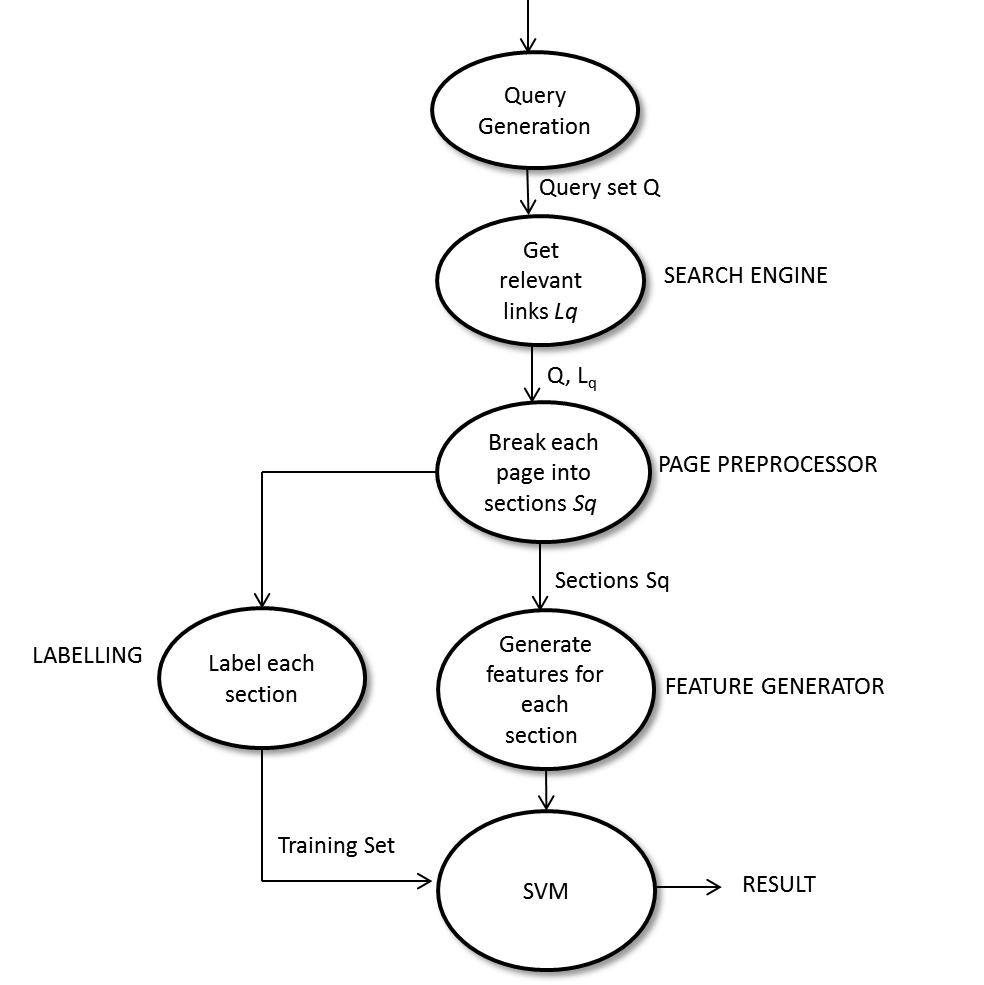
\includegraphics[width=0.80\textwidth]{./architecture}\\
\end{center}

\section{Prototype}

With regards to programming language in which we will implement the project, we have chosen \textit{JAVA} as the language of choice owing to the availability of well supported classes to implement SVMs and the object-oriented features in general.

We have made a prototype program with placeholder stub functions for each component. Currently each stub does no useful work but just passes the data along.

Each component can be individually developed and further refined to produce the optimal output.

%----------------------------------

\chapter{Design Details}

\section{Query Generation}

\begin{itemize}

	\item Take the topic \textbf{t} as input.
	\item Generate set \textbf{T} of related subtopics and add the topic to \textbf{T} as well.
	\item Query Set \textbf{Q} := \textbf{T} x \{`questions', `problems', `solved examples'\}.

\end{itemize} 

Firstly, we will take the input of the topic and generate a list of sub-topics and other keywords which relate to the topic. For eg. if the topic is `Operating Systems', various sub-topics can be `Processes', `Threads', 'Cache' etc. These will form the set \textbf{T}.

Each phrase in \textbf{T} will be appended with chosen suffixes such as \textit{questions} and \textit{problems} to generate the query set Q which will be queried on the search engine.

\section{Search Engine}

$\forall \textbf{q} \in \textbf{Q}$ :

\begin{itemize}

	\item Search the internet for the query phrase \textbf{q} using Google Custom Search API (or any other search engine).
	\item Add the top \textit{nLinksPerQuery} links to set \textbf{$L_{q}$}.

\end{itemize}

\section{Page Preprocessor}

$\forall \textbf{l} \in$ \textbf{$L_{q}$} :

\begin{itemize}
	\item Load the link \textbf{l} in the Lynx browser. This will strip away all markup data, images etc. and yield only the text portions.
	\item The text of the page is then broken up into sections on the basis of - \\
	\begin{itemize}
		\item Number of lines
		\item Paragraph Structure
		\item Interrogative Indicators - \textit{`what', `how', `explain', `define', `?', `elucidate'} etc.
	\end{itemize}
	\item Each section \textbf{s} thus obtained is added to the section set \textbf{$S_{q}$}.
\end{itemize} 

For each query phrase \textbf{q} $\in$ \textbf{Q}, we will load each link we have in our link set \textbf{$L_{q}$} in the Lynx browser to strip it of all useless markup data, links and pictures and parse out only the text portions available on the page which may contain the questions. 

Each page will then be broken into various sections. This will be done by a parser which will determine \textit{good} sections which may be questions on the basis of a maximum number of lines, the paragraph tags of html and interrogative indicators like a line ending with a \textit{`?'} or lines starting with words like \textit{`what', `define'} etc. as these are likely to be starting or ending words of a question.

Each section \textbf{s} thus obtained will be added to the section set \textbf{$S_{q}$} for a query.

\section{Feature Generator}

The feature generator will generate the features and statistics for each subsection, which will be analysed by the SVM to create the regression model. 

We adapt the first three features from \textit{SQUINT} to determine the relevance of a section to the query phrase\cite{squint}. 

Furthermore, we propose two additional features to determine whether a section contains a question or not. \\

The features are ---

\begin{enumerate}
	\item Word Rank Based Feature
	\item Bigram Rank Based Feature
	\item Coverage of Top Ranked Tokens
	\item Coverage of Interrogative Indicators
	\item Absence of Specific Keywords
\end{enumerate}


\subsection {Word Rank Based Features}

The rank of a word is defined to be its position in the list if the words were ordered by frequency of occurrence in \textbf{$S_{q}$}.\cite{squint}

We would have a feature each for say, the top 200 most frequent words in \textbf{$S_{q}$}. 

For the $i^{th}$ ranked word, this feature would basically have the value for the frequency of this word in the current section. 

We can limit the dimensionality of the input vector by bucketing words by a certain range of ranks. 
For example, we can bucket ranks 1-5, 6-10, 11-15...etc to aggregate word counts, and come up with a feature vector of reduced dimensionality. 

We also normalize for the length of the section since we do not want to be biased towards long sections.

The optimal number of words and the bucket size needs to be determined experimentally.

\subsection {Bigram Rank Based Features}

A bigram is defined to be two consecutive words occurring in a section.\cite{squint}

This feature is computed in a manner similar to the previous set of features. 

This feature is based on the intuition that the correlation between two words might be more informative than the words taken individually. For instance, `machine learning' suggests a stronger relation to a query `AI SVM' than the
individual words `machine' or `learning'. 

For this feature as well, we will adjust the dimensionality by bucketing and limiting coverage of ranks depending on experimental results.

\subsection {Coverage of Top Ranked Tokens}

Relevance to a topic may also be captured by the coverage of top ranked token types in the section.\cite{squint}

For example, if we have a bucket size of 5, we might be interested in knowing how many of the top 5 ranked words occur in this section, how many of the next 5 highly ranked words occur in this section and so forth. 

Specifically, if the top 5 ranked token types are `learning', `machine', `data', `access', and `database', and a section contained `learning' and `data', the corresponding value for this feature is 2.

\subsection {Coverage of Interrogative Indicators}

Presence of words such as \textit{`what', `why', `explain', `define', `elucidate'} etc. are strong indicators that the section contains a question. 

Thus we propose this feature whose value is the coverage of a predefined set of such interrogative indicators present in the section.

We need to experimentally determine whether the frequency or coverage of interrogative indicators is a better feature.

\subsection {Absence of Specific Keywords}

There are certain words or patterns, the presence of which strongly indicate a section of text to not have a question. 

For example, if a sentence begins with a \textit{`Yes'} or \textit{`No'}; or certain words like \textit{`because'} are present, there is a high chance that the section is not a question. 

We check for the coverage of such words in the section using a pre-defined list. 

This feature is used as a negative feature as a higher value indicates a lower probability of the section being a question.

\section{Labelling (Training Set Generation)}

For generating the training set, we will manually label a set of sections as to whether they are relevant questions of the given topic or not and this data will be used to train the SVM to generate the model. 

\section{Support Vector Machine}

We will use a Support Vector Machine with a Linear Kernel as recommended by Joachims\cite{joachims}.

This component will be trained using the Training Set comprising of the section sets with the generated feature vectors and manually tagged labels. The training data will be analysed to generate a regression model. \\

During the real runs of the application, the model generated during training will be used by the SVM to identify the relevant sections and tag them appropriately. 

The sections tagged as `relevant' will be added to the result set \textbf{R}.\\

\section{Output}

The output component will take all the sections tagged as `relevant question' present in set \textbf{R} and output them in a clean format.

%---------------------------------------------------

\chapter{Further Work}

While the overall architecture of the application seems promising, we need to find out the exact parameters for each section which will produce the best results. This can be only determined experimentally once the programming part of the project is completed. \\

Over the course of the next semester, we will first finish coding the application with configurable parameters. We will then tune the parameters and refine each component by performing iterations of training, testing and validation. \\

Analysis of which features are actually useful and the weightage of each feature in determining whether a section is a question relevant to the input topic needs to be determined experimentally. 

During the course of implementation and analysis, we may also consider other features which correlate to a section's relevance. \\

We will continue to follow the latest research related to machine learning in order to incorporate any suitable developments. \\

%------------------------------------------------------------------------

\clearpage
\addcontentsline{toc}{chapter}{References}
\begin{thebibliography}{99}

\bibitem{squint} SQUINT - SVM for Identification of Relevant Sections in Web Pages for Web Search, \textbf{Riku Inoue, Siddharth Jonathan J.B., Jyotika Prasad}, \textit{Department of Computer Science, Stanford University}

\bibitem{teevan} The Perfect Search Engine is Not Enough : A Study of Orienteering Behavior in Directed Search, \textbf{Jaime Teevan, Christine Alvarado, Mark S. Ackerman and David R. Karger}, \textit{Proceedings of the SIGCHI conference on Human factors in computing systems. pp. 415-422, April 2004.}

\bibitem{wikiML} Wikipedia article on Machine Learning, http://en.wikipedia.org/wiki/Machine\_learning

\bibitem{elements} The Elements of Statistical Learning: Data Mining, Inference, and Prediction, \textbf{Trevor Hastie, Robert Tibshirani, Jerome Friedman}

\bibitem{joachims} Text Categorization with Support Vector Machines: Learning with Many Relevant Features, \textbf{Thorsten Joachims}, \textit{Universitat Dortmund, Informatik LS8, Baroper Str. 301, 44421 Dortmund, Germany}

\bibitem{wikiSVM} Wikipedia article on Support Vector Machine, http://en.wikipedia.org/wiki/Support\_vector\_machine

\bibitem{wiki} Machine Learning, http://en.wikipedia.org/wiki/Machine\_Learning

\bibitem{coursera} Machine Learning Course on Coursera, https://class.coursera.org/ml-2012-002/class/index

\end{thebibliography}

%----------------------------------------------------------------------

\end{document}
